\section{Bilder Konzeptionierung}\label{sec:bilder-konzeptionierung}

\begin{figure}[htbp]
    \centering
    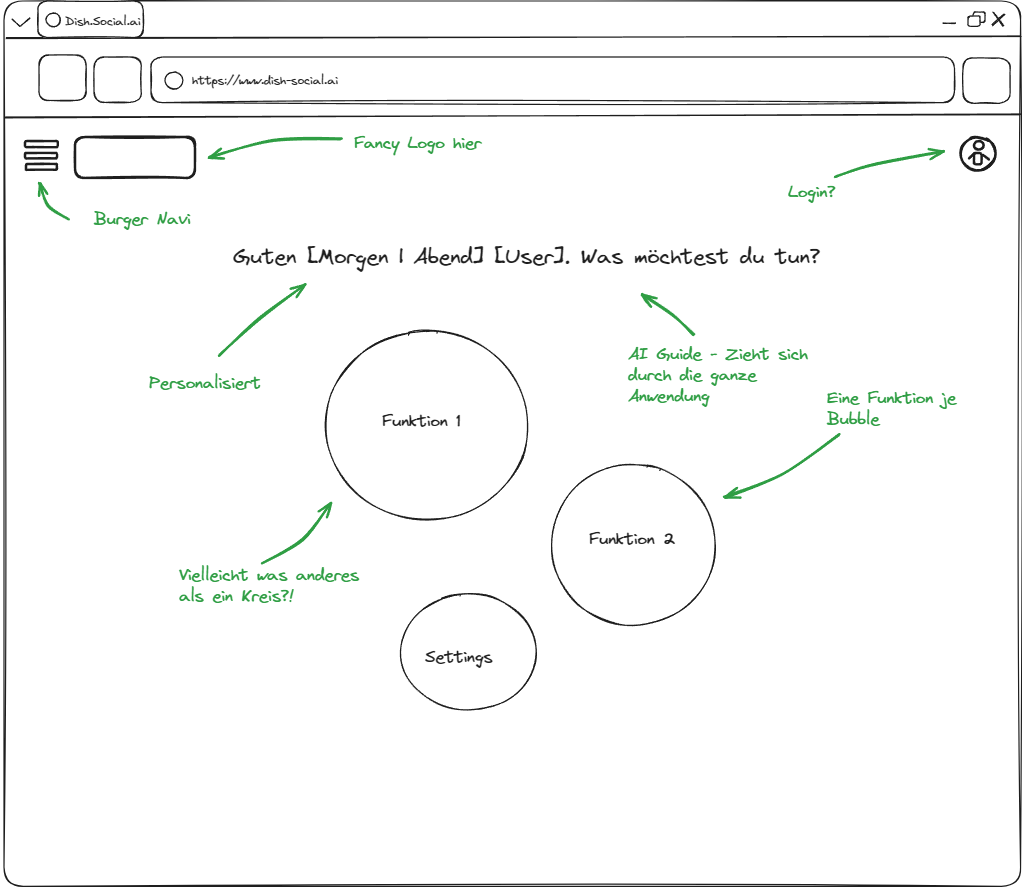
\includegraphics[width=\textwidth]{abbildungen/Konzept/Konzept Landing Page}
    \caption[]{Konzept Landing-Page Darstellung}
    \label{fig:landing-page-concept}
    \raggedright Quelle: Eigene Darstellung
\end{figure}
\newpage

\begin{figure}[htbp]
    \centering
    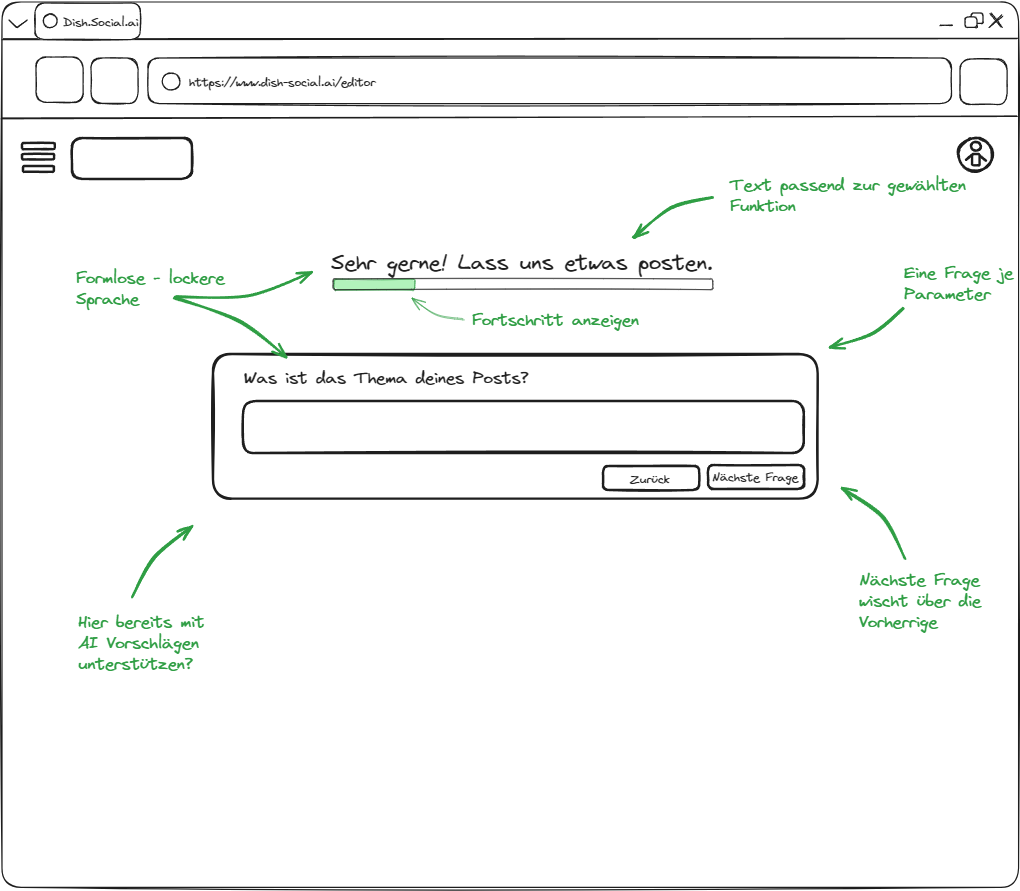
\includegraphics[width=\textwidth]{abbildungen/Konzept/Konzept Dialog}
    \caption[]{Konzept Dialog Darstellung}
    \label{fig:dialog-concept}
    \raggedright Quelle: Eigene Darstellung
\end{figure}
\newpage

\begin{figure}[htbp]
    \centering
    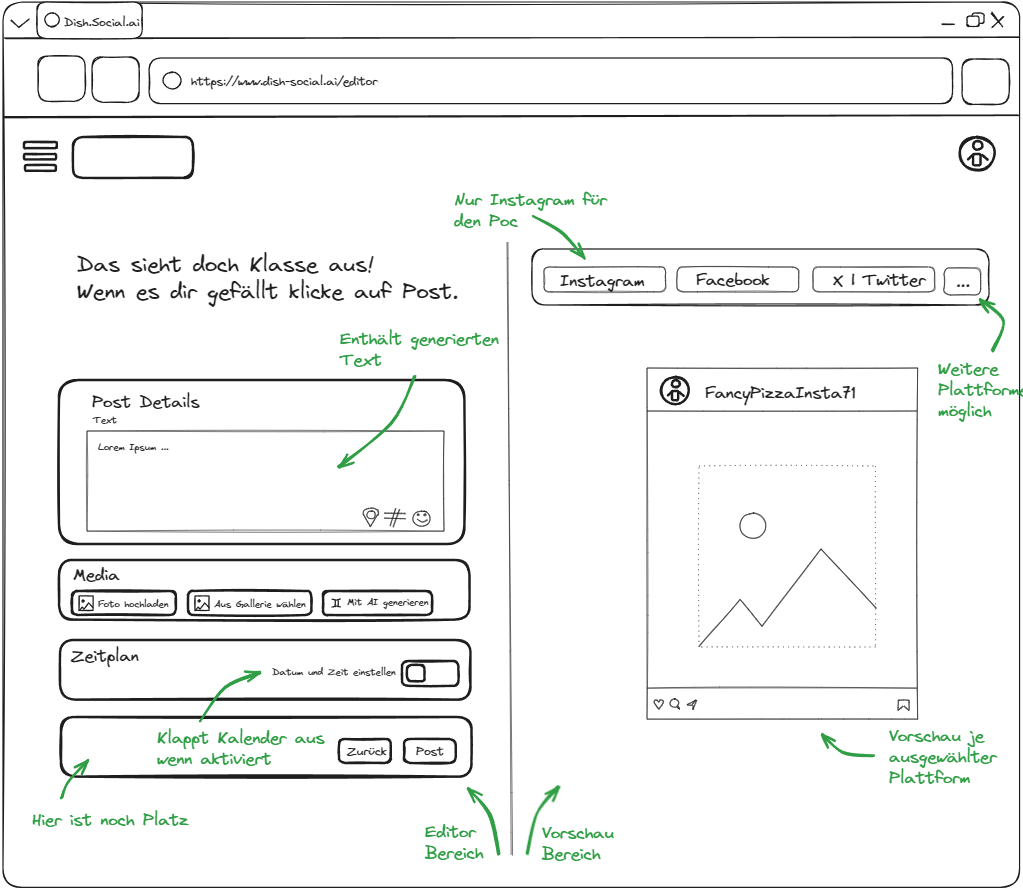
\includegraphics[width=\textwidth]{abbildungen/Konzept/Konzept Editor}
    \caption[]{Konzept Editor Darstellung}
    \label{fig:editor-concept}
    \raggedright Quelle: Eigene Darstellung
\end{figure}
\newpage

\begin{figure}[htbp]
    \centering
    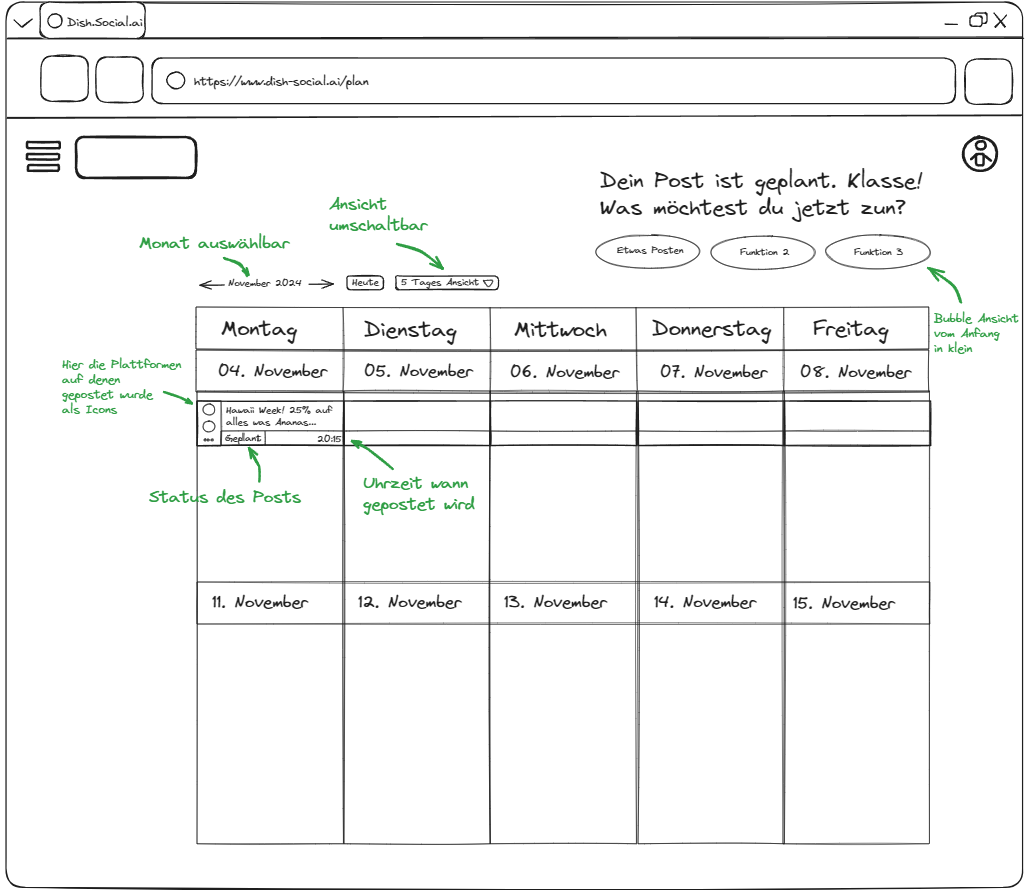
\includegraphics[width=\textwidth]{abbildungen/Konzept/Konzept Kalender}
    \caption[]{Konzept Kalender Darstellung}
    \label{fig:calendar-concept}
    \raggedright Quelle: Eigene Darstellung
\end{figure}
\newpage

\section{Bilder Figma Design}\label{sec:bilder-figma-design}
\begin{figure}[htbp]
    \centering
    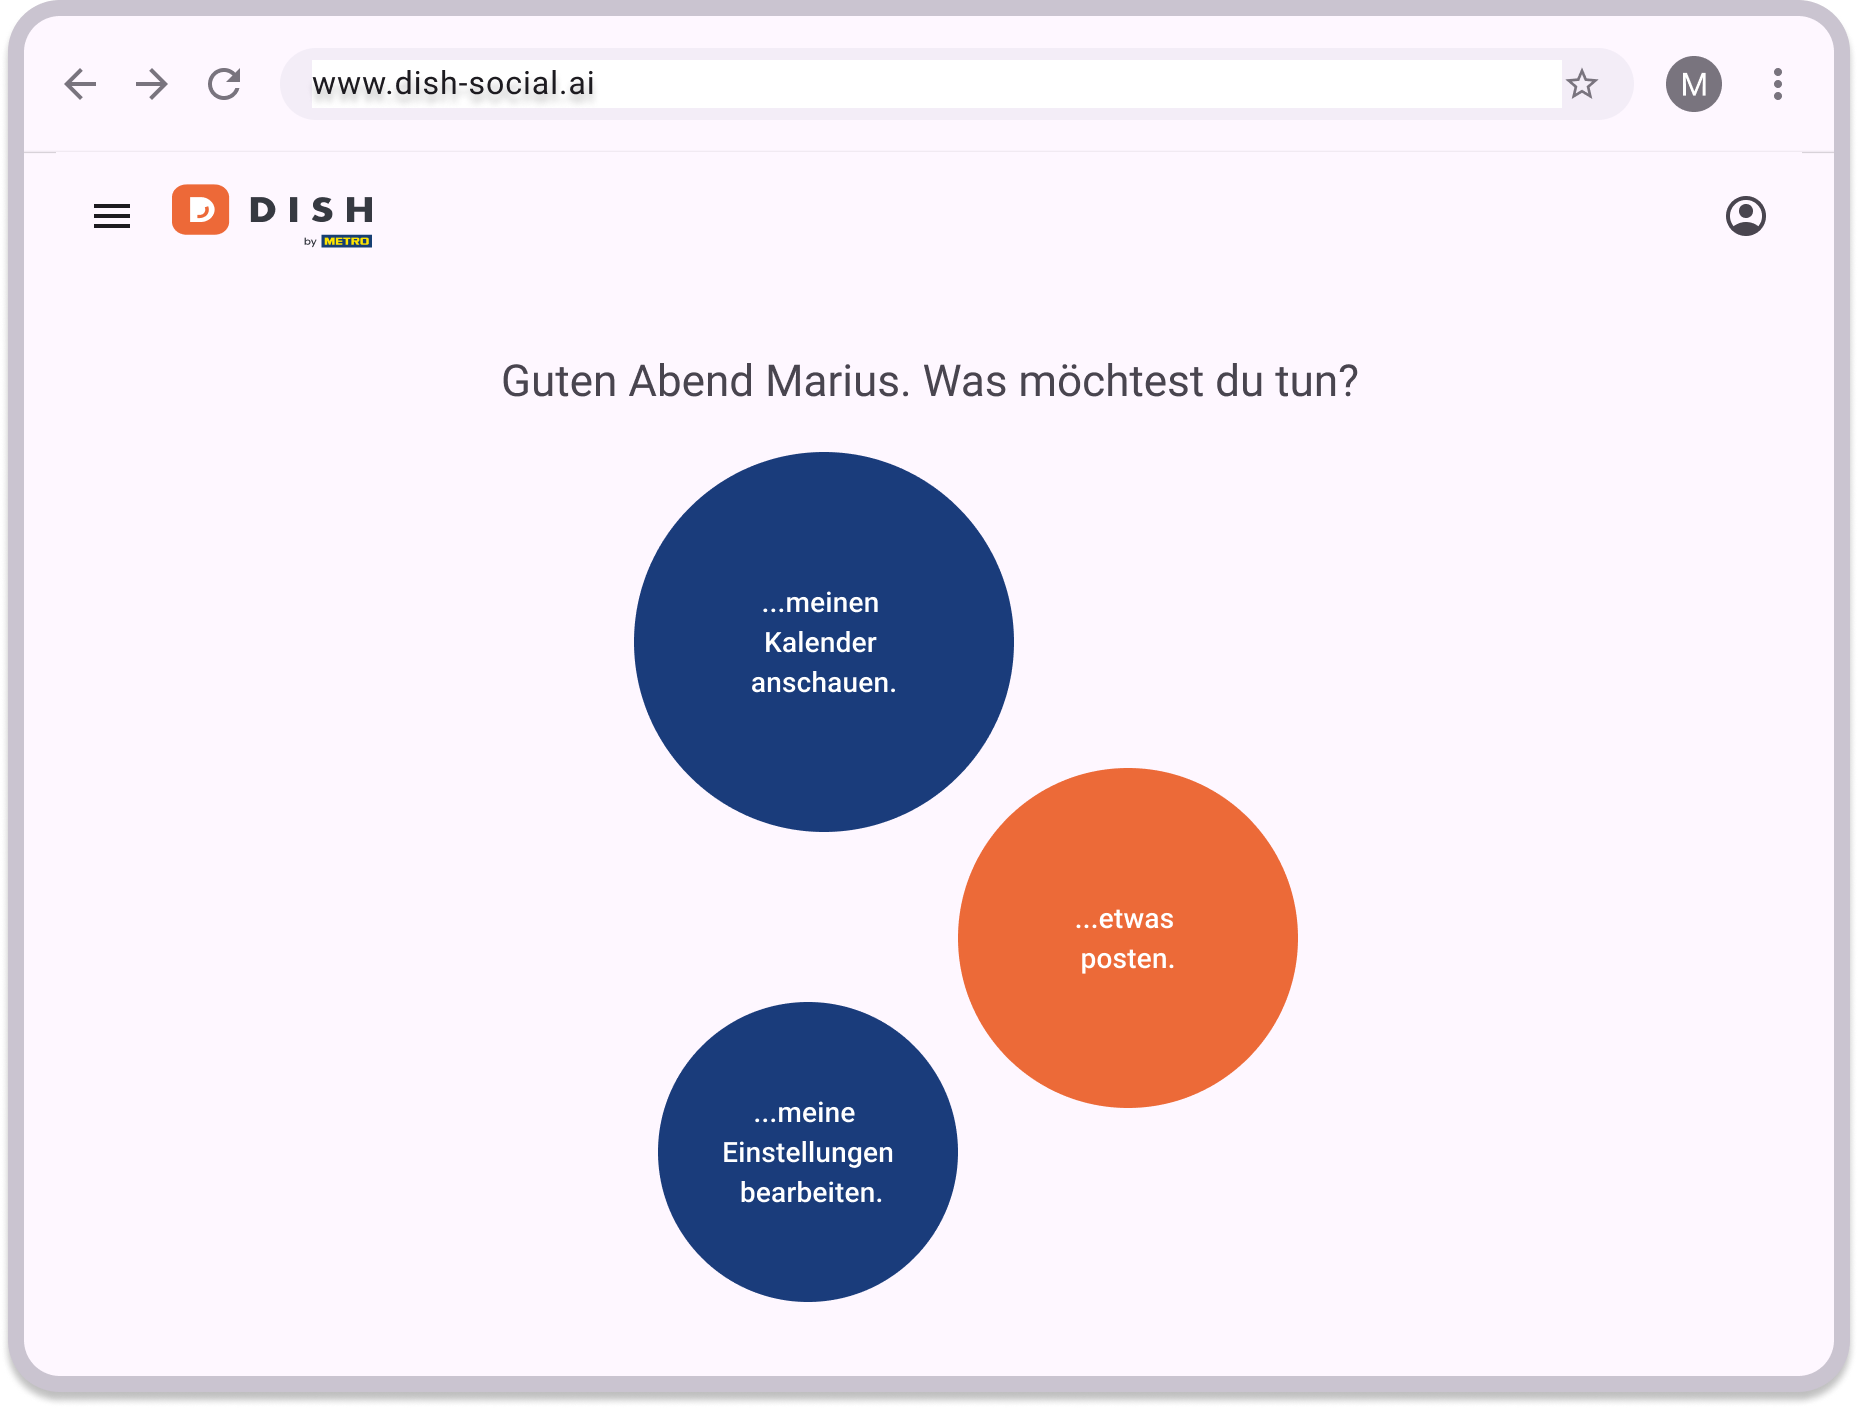
\includegraphics[width=\textwidth]{abbildungen/figma/Landing Page}
    \caption[]{Figma Design Landing-Page Darstellung}
    \label{fig:landing-page}
    \raggedright Quelle: Eigene Darstellung
\end{figure}
\newpage

\begin{figure}[htbp]
    \centering
    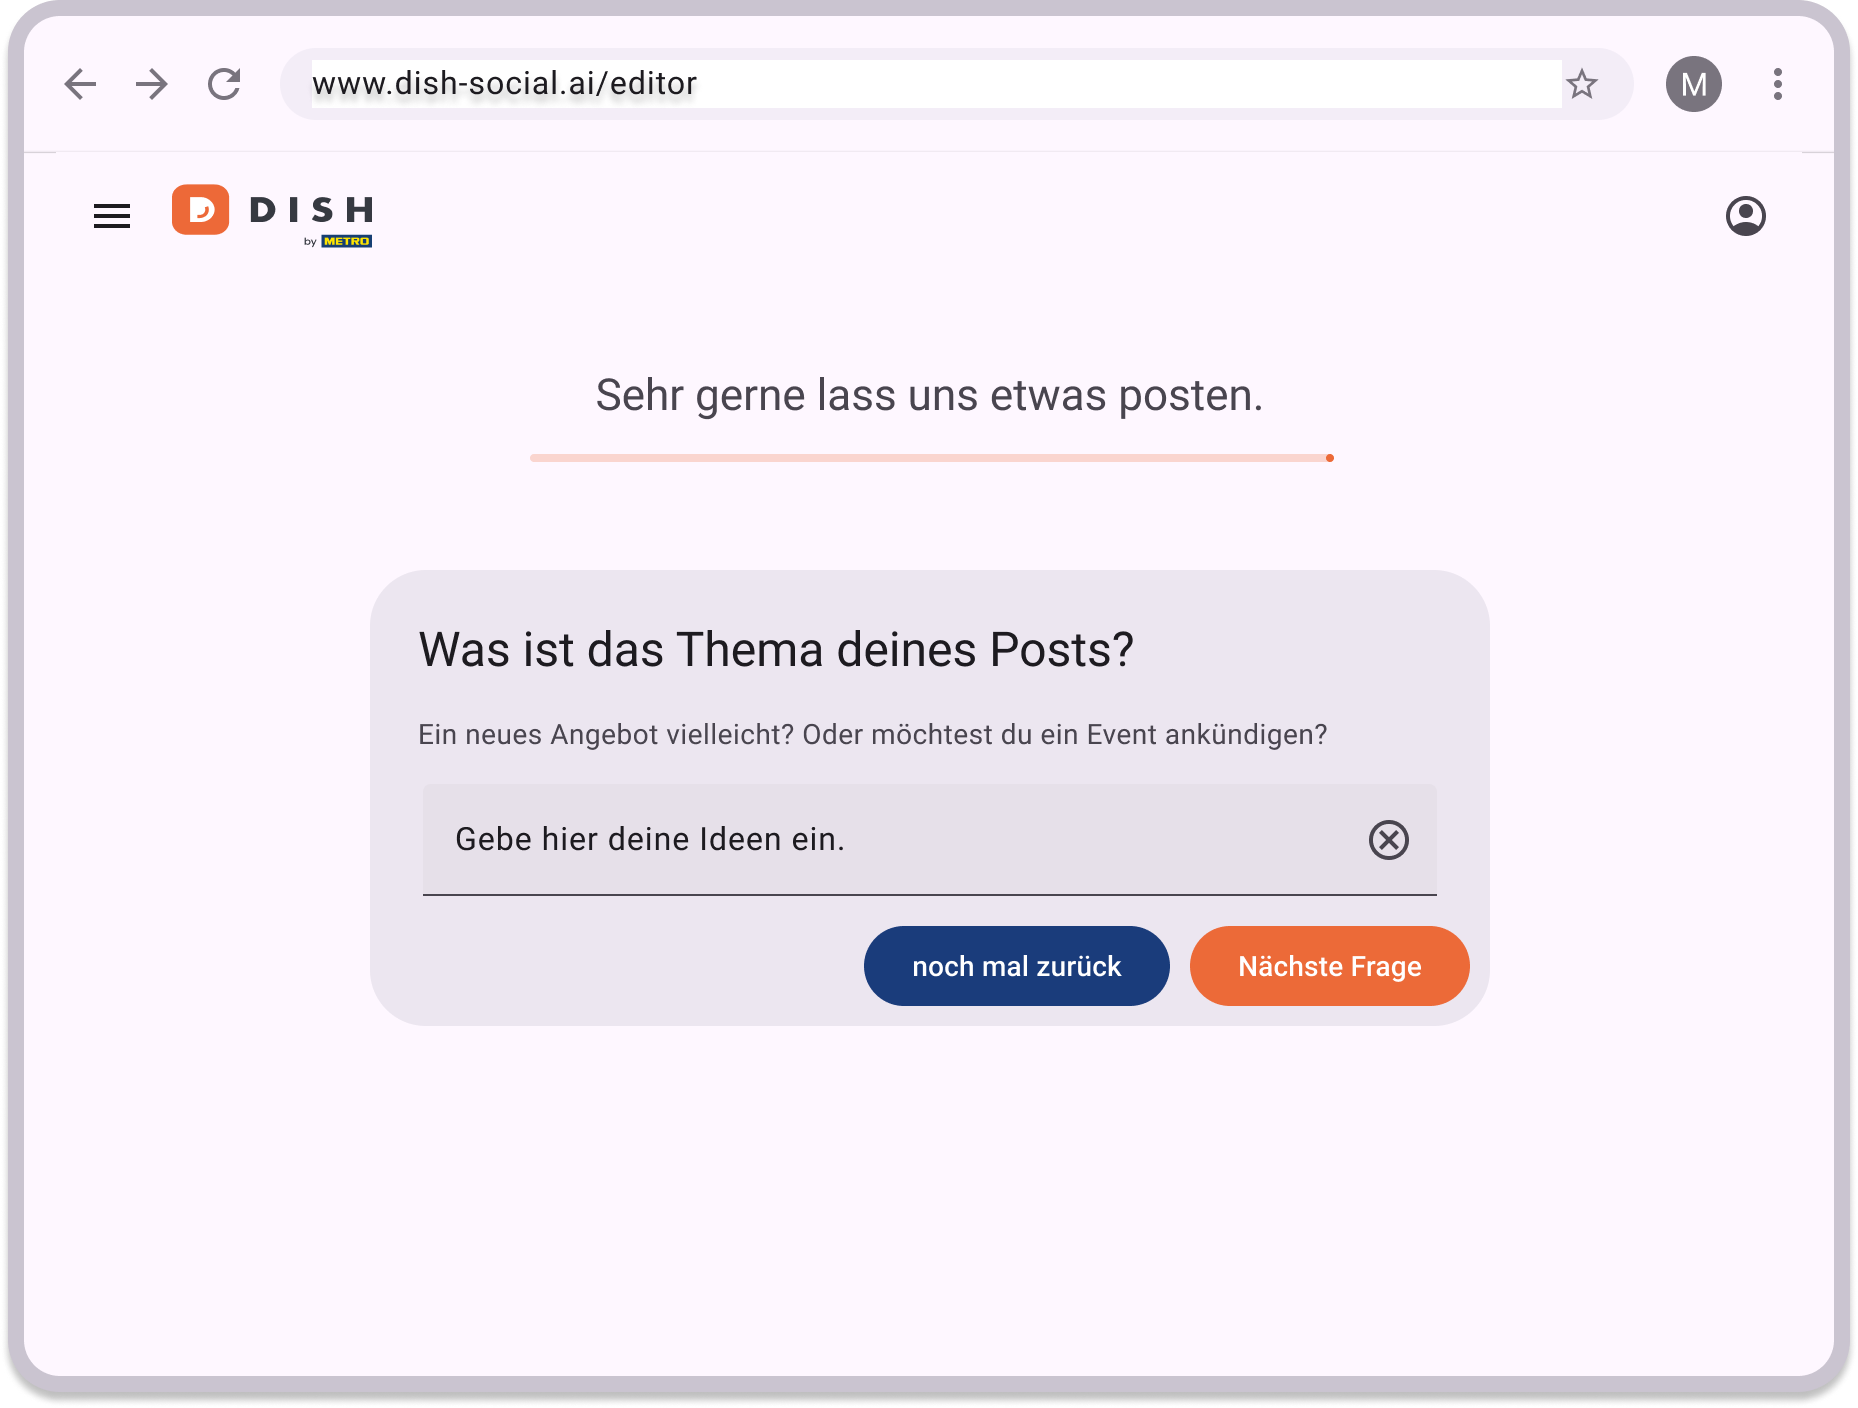
\includegraphics[width=\textwidth]{abbildungen/figma/Dialog}
    \caption[]{Figma Design Dialog Darstellung}
    \label{fig:dialog-page}
    \raggedright Quelle: Eigene Darstellung
\end{figure}
\newpage

\begin{figure}[htbp]
    \centering
    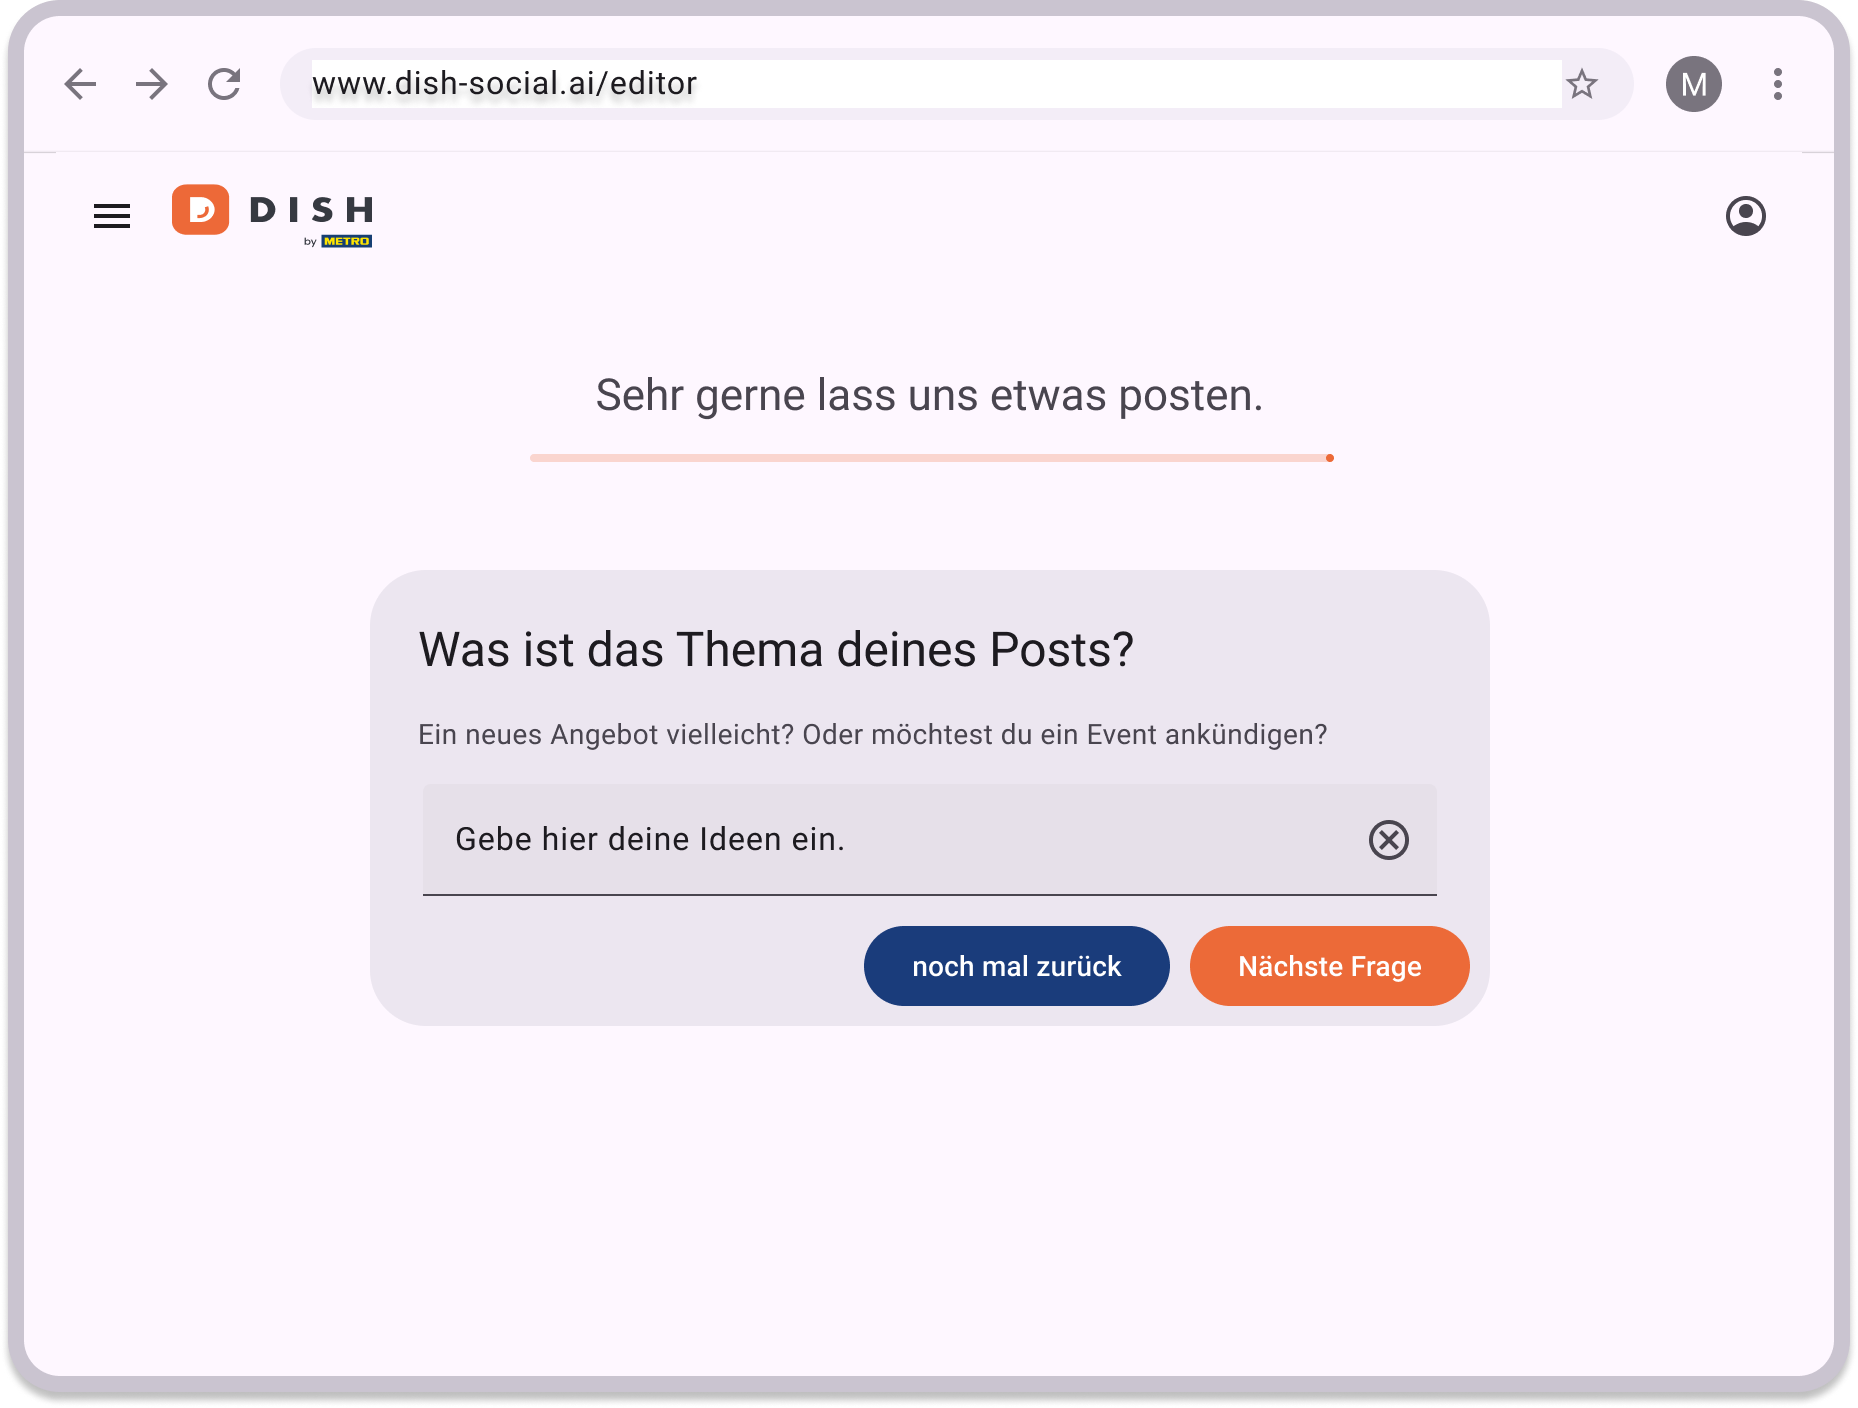
\includegraphics[width=\textwidth]{abbildungen/figma/Editor}
    \caption[]{Figma Design Editor Darstellung}
    \label{fig:editor-page}
    \raggedright Quelle: Eigene Darstellung
\end{figure}
\newpage

\begin{figure}[htbp]
    \centering
    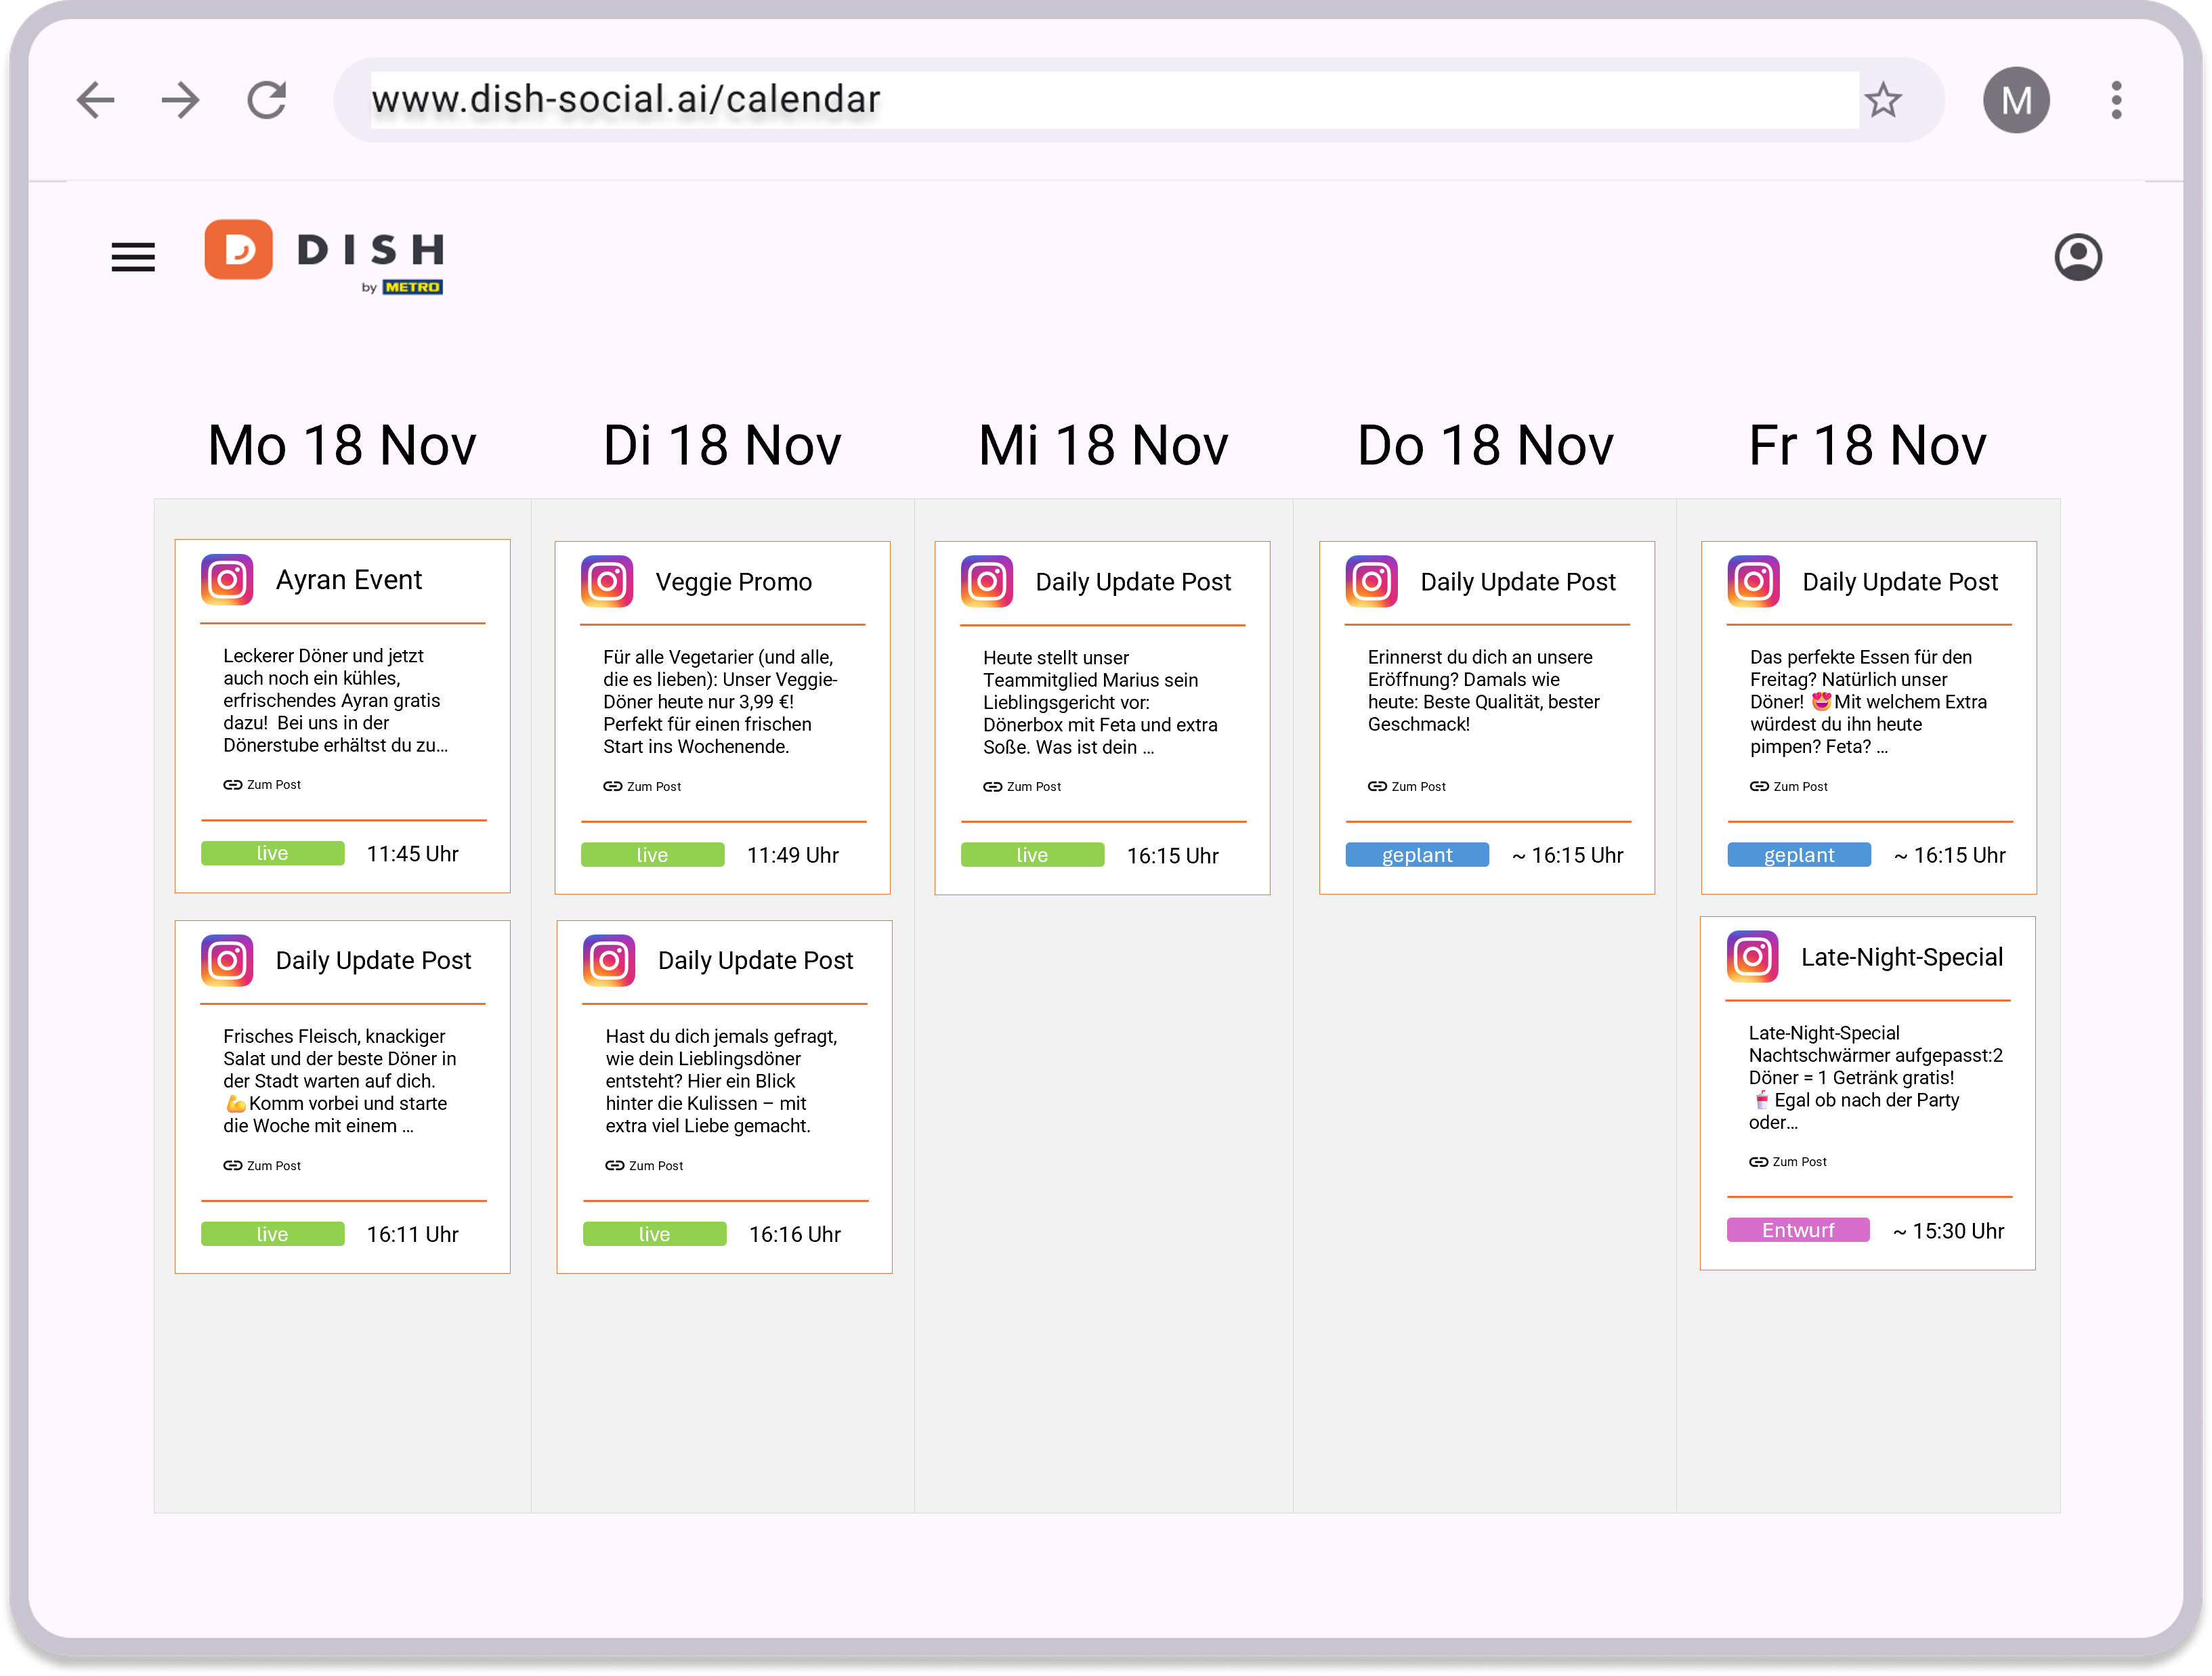
\includegraphics[width=\textwidth]{abbildungen/figma/Kalender}
    \caption[]{Figma Design Kalender Darstellung}
    \label{fig:calendar-page}
    \raggedright Quelle: Eigene Darstellung
\end{figure}

\section{Ergebnisse der Textgenerierung}\label{sec:bilder-textergebnisse}

\begin{figure}[htbp]
    \centering
    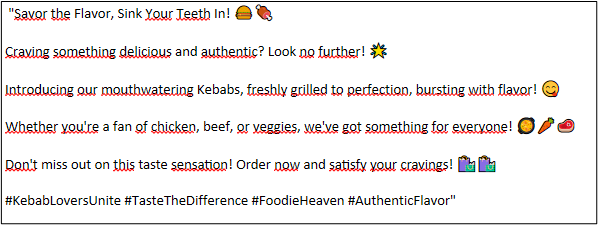
\includegraphics[width=\textwidth]{abbildungen/textresult_mistral}
    \caption[]{generierter Text durch das Text-to-Text Modell mistralai/Mistral-7B-Instruct-v0.3}
    \label{fig:textresult_mistral}
    \raggedright Quelle: Eigene Darstellung
\end{figure}

\begin{figure}[htbp]
    \centering
    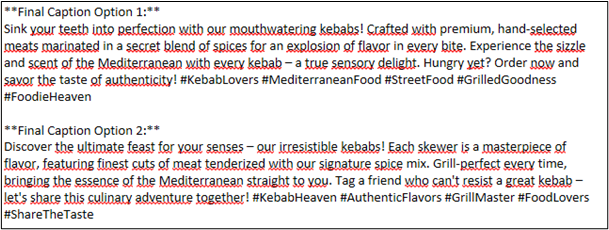
\includegraphics[width=\textwidth]{abbildungen/textresult_Qwen}
    \caption[]{generierter Text durch das Text-to-Text Modell Qwen/QwQ-32B-Preview}
    \label{fig:textresult_Qwen}
    \raggedright Quelle: Eigene Darstellung
\end{figure}

\begin{figure}[htbp]
    \centering
    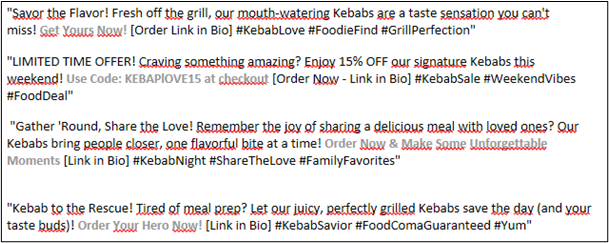
\includegraphics[width=\textwidth]{abbildungen/textresult_nvdia_nemotron}
    \caption[]{generierter Text durch das Text-to-Text Modell nvidia/Llama-3.1-Nemotron-70B-Instruct-HF}
    \label{fig:textresult_nvdia_nemotron}
    \raggedright Quelle: Eigene Darstellung
\end{figure}
\clearpage
